\chapter{Methods} \label{methods}
This Chapter contains a thoroughly description with rationales of the research methods adopted by this thesis work. Firstly, a characterization of the case is provided. It contains the description of the settings, the case itself and the units of analysis. Subsequently, the focus shifts to the methods and sources through which the data has been collected. For every different source the text describes where applicable use cases and rationale. Finally, the chapter ends with an explanation of the data analysis methods used. 


%
%
% START CASE DESCRIPTION
%
%
\section{Case Study design}	\label{sec:case-description}
Yin \cite{case_study_guide} defines case studies as \textit{``an empirical enquiry that investigates a contemporary phenomenon within its real-life context, especially when the boundaries between phenomenon and context are not clearly evident.''}
Furthermore, as reported by Runeson et al. \cite[p.~3]{case_study_software_engineering}, \textit{``Case studies do not generate the same results on, for example, causal relationships, as controlled experiments do, but they provide a deeper understanding of the phenomena under study''}. Therefore, considering the setting of this study and its aim, this research methodology is the most suitable to answer the research questions listed in Section \ref{sec:introduction}.

Precisely, this study will use the \textit{multiple, holistic case study} design defined by Yin \cite{case_study_guide} and displayed in Fig. \ref{fig:case-study-types}. Furthermore, given the weak body of knowledge (see section \ref{sec:related_work}) this Thesis also includes the exploratory variant. This choice is supported by \cite[p.~19]{case_study_software_engineering}: \textit{``.For exploratory research questions, the case study strategy is a perfect match''}.

However, to counter the criticisms moved to this methodology \cite[p.~4]{case_study_software_engineering}, a rigorous approach is needed. For this reason, the guidelines expressed by the Runeson et al.\ \cite{case_study_software_engineering} are taken into consideration thoroughly. They specifically target the Software Engineering field providing a detailed checklist contained in Appendix \ref{checklist_for_case_studies} with embedded links to the relevant parts of this report. Additionally, the case study reference proposed by Yin \cite{case_study_guide}, which doesn't constrain the scope to a precise field, is used.


For adequately characterize the Case under study Yin \cite{case_study_guide}, suggests to describe 1) the context in which the Case is, 2) the Case itself, and 3) the Units of Analysis. However, as Fig. \ref{fig:case-study-types} shows, when applying the holistic design cases and units of analysis are equivalent. Therefore, the following sections report the generic context and cases with their particular contexts.

\begin{figure}[hbt]
    \centering
    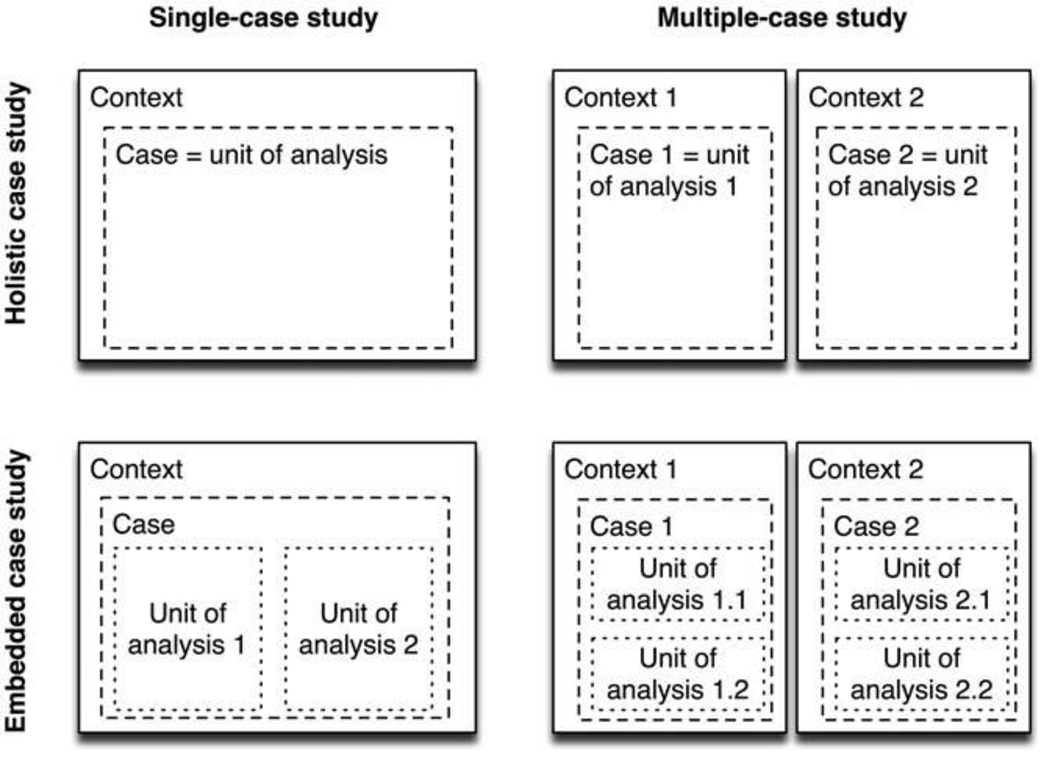
\includegraphics[width=\textwidth]{figure/yin-case-studies.pdf}
    \caption{Yin \cite{case_study_guide} possible case studies configuration.}
    \label{fig:case-study-types}
\end{figure}


\subsection{The generic context}

This study took place in the Swedish office of the Company, a fictional name used to indicate a real entity that globally counts more than 3000 employees scattered in several offices. Its core business is licensing software products for managing personnel and equipment in the context of Transportation. Their portfolio offers different solutions to cover several business needs in terms of short or long term planning, personnel optimization, etc.

Internally, teams use Scrum for managing their development activities. They have considerable freedom in choosing sprint length, and the Definition of Done, which is built atop of a minimum one provided by the parent company. Teams are cross-functional and hence contain people with different areas of expertise; they also are self-contained meaning that they should carry out all software related activities independently.

This last fact is of great relevance to this study. In fact, all testing activities are carried on separately, following the minimum guidelines expressed in the Definition of Done. However, this lenient artifact causes teams to use different testing strategies for complying with the testing pipeline. Therefore, there is a chance to analyze TD accruing in various projects. 

As shown in Fig. \ref{fig:testing_pipeline}, this pipeline is composed of four levels (lower to higher): unit tests, components tests, system tests, end to end tests. These levels do not differentiate between functional and quality (non-functional) testing types as these can take place at any level. 

Notably, unit tests are carried on by developers alongside development activities and aim to test the System at function and class level. Therefore, there is a high number of them and tend to be fast to execute and relatively simple. At this level, developers follow the same guidelines specified for the actual source code, with the sole exception that, according to the minimum definition of done, they are not reviewed. Above in the hierarchy, there are component tests that target the interaction between macro software entities and aim to ensure that the sub-parts of the system deliver the desired functionality. At this level, tests target the exposed APIs and not the internal mechanics of the source code. The next level in the pipeline, System level tests, aims to assure that user functionality and business processes of a single system comply with the specification. These tests execute at user interface level with realistic data sets and possibly data volume. Finally, End to End tests are similar in concept and execution to System tests, but they test the interaction of two or more complete systems. Furthermore, these levels can be further divided into functional and non-functional tests, which respectively target functionality and quality attributes of the system.

Finally, the two middle layers of the pipeline contain test that can be semantically divided into two groups: smoke tests and regression tests. The former group contains simpler tests that control the behavior of macro functionality, e.g.\ a window is displayed if the new window button is pressed. The latter group, instead, includes tests that represent use-case scenarios and hence more detailed and complicated. The following sub-section provides additional information on the topic.

\todo{Improve figure \ref{fig:testing_pipeline} readability}
\todo{Extract the image from the testing chapter document}

\begin{figure}[hbt]
    \centering
    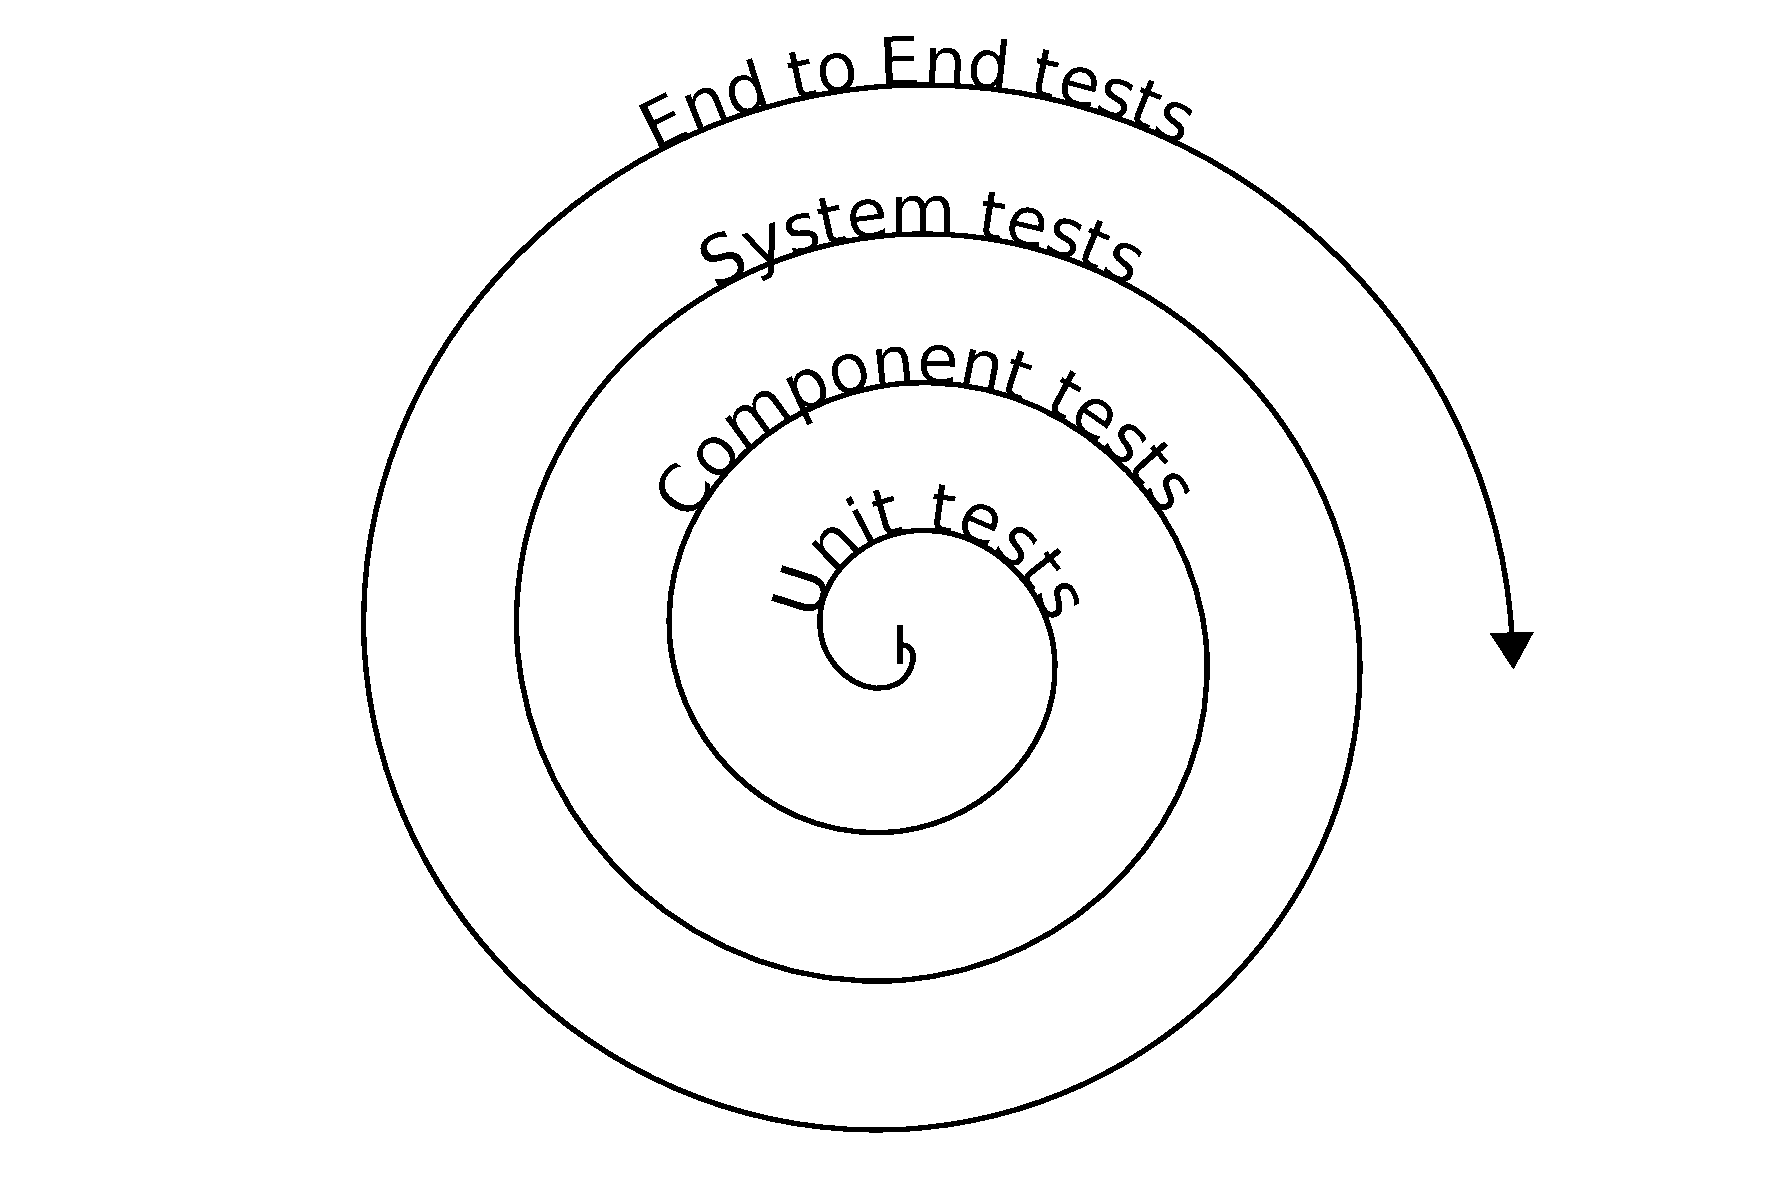
\includegraphics[width=\textwidth]{figure/testing_pipeline.pdf}
    \caption{Testing pipeline in use at the Company}
    \label{fig:testing_pipeline}
\end{figure}

\subsection{Cases definition and units of Analysis}

Among the ongoing projects at the Company, this study will inspect the accretion of TD in projects using Hewlett Packard's Unified Functional Tests (UFT) to test user interfaces. Precisely, there are two projects meeting this requirement and will be called Project A and B in the rest of the document.

Both projects have associated two unique repositories, one for Smoke Testing and another one for Regression Testing. Furthermore, there are two shared repositories that contain common methods and functions used by test scripts. For this reason, considering the substantial difference in purpose of such repositories they are considered separately. Therefore, the label \textit{Project D} is used to group them within an abstract entity that does not map to any real active project.


\subsubsection{Project A}
This project is the new solution developed to replace the legacy Project B. It is Java based and the client runs on the Windows operating system.

\subsubsection{Project B}
Project B is a tool used for registering and handling passengers. It register who is on-board of which airplane and so forth. This tool is less customizable than project A, but it is a more critical part of the Ecosystem. In fact, international rules require a constant monitoring of airplanes' passengers. The client and server are monolithic and the client is run on clients that allow to run Unix X-sessions from other operative systems.

\subsubsection{Project C}
Project  consist of a highly customizable software used to manage crew personnel both in the short and long term. The client runs on Windows and it is realized with Java.

\subsubsection{Project D}
As mentioned before, Project D consists of two repositories that contain generic functions used by test suites. These tie UFT tests with the Windows operating system. They allow to kill and spawn a process, create and read files, etc. Furthermore, they also create skeleton for the report engines; they are used to create summaries of test runs in different formats such as HTML, XML, etc.

%
%
% END CASE DESCRITPION
%
%

%
%
% START DATA GATHERING
%
%
\section{Data Gathering}
As recommended by \cite{case_study_guide,case_study_software_engineering}, data has been gathered from various sources in order to increase Data Triangulation and hence improve the reliability of the study. These sources are: 1) informal interviews (a.k.a.\ coffee machine / water bowl interviews), 2) the company´s forum, 3) the company´s issue tracker and backlog, 4) the repositories of the relevant project, and 5) semi-structured interviews.

\todo{Mention that I used both quantitative and qualitative sources for improving reliability}

\subsection{Informal Interviews}
As stated by Milberg and Strang \cite{informal_interview} researchers should strive to attain qualitative data from various sources in order to gain a well-rounded knowledge of the phenomenon under study. For this reason, this study also collected information from Informal Interviews.

This source helped defining the scope of the inquiry in the first stages of the study by identifying at very high-level main problems and triggering causes. However, due to the lack of repeatability associated with this method, such data has not been used for sensitive parts of the study like theory validation.

In fact, frequency, location, and interviewees were random. Furthermore, as highlighted by McNamara \cite{general_guidelines_for_interview}, this kind of inquiry is not steered by schemes, but instead affected by the interaction between participants. Moreover, they occurred during lunch and coffee breaks whenever possible, and bootstrapped by current issues encountered by the interviewee. Apparently a not controlled environment. However, their importance during the first phases of this Thesis is clear since they focused the attention on important parts, sources, and documentation.

\subsection{Mining of The Forum} \label{mining_forum}
In order to enable Knowledge Sharing the company adopted Confluence, a collaborative software / forum developed and maintained by Atlassian\texttrademark\. It allows technical and non-technical employees to share procedures, ideas, and comments in an asynchronous fashion, and, for this reason, this source is valuable since it contains numerous information, which can shed light on the problems this Thesis aim to study.

However, considering the magnitude of the available data, it was important to ensure that the mining did not miss any information. Therefore, it has been performed through a systematic approach using the embedded search engine provided by the tool and two manual filtering steps. In fact, the system contains data covering several years and include several thousand discussions threads and many more answers. 

The keywords entered in the search engine were included in double quotes in order to enable the \textit{exact match} feature. This choice was needed to limit the number of results to a manageable size. For instance, \textit{test maintenance} yielded 8467 results whereas \textit{"test maintenance"} 28. Subsequently, the first coarser temporal based filter followed. It eliminated hits older than one year. Next, the second finer filter based on the relevance was used. Finally, the remaining set of posts has been carefully read, and pertinent ones have been anonymized and transcribed in the Thesis database.

This paragraph reports the rationale connected with the first filtering activity. The temporal time frame is narrow for two reasons. Firstly, the test-ware stack changed during last year (2014) and hence the findings could be biased by information not relevant or tied to the old technologies. Secondly, the mortality of the resources has been taken into account. In fact, the Company greatly relies on consultants, and their turnover is shorter than typical employees. 

\subsection{Mining of The Issue Tracker / Backlogs} \label{mining_issue_tracker}
The Company uses an all in one solution for managing issues and their Agile Environments: JIRA and JIRA Agile Plugin. These tools are also supported by Atlassian. Similarly to the forum, this source contains a high number of entries that have been mined to provide insights regarding the problems under analysis.

This activity has been carried on firstly with a parsing script \footnote{\href{https://github.com/MMMarcy/JiraMiner4Thesis}{https://github.com/MMMarcy/JiraMiner4Thesis}} that, after parsing the JSON file generated through the JIRA Rest APIs \footnote{\href{https://developer.atlassian.com/jiradev/api-reference/jira-rest-apis}{https://developer.atlassian.com/jiradev/api-reference/jira-rest-apis}}, created a spreadsheet with the relevant data of choice.

\todo{Use URL shortener}

The filtering process used the JQL query language, which is supported natively by the APIs mentioned above. The data clause targeted by the query was \textit{text}, which is a macro field that includes issue's name, description, summary, and comments. Regarding the keywords used, they were tested in a trial  and error fashion. However, the process showed that the query using a boolean or with \textit{``UFT''} and \textit{``QTP''} yielded the best combination of relevant results.

The spreadsheet contains some statistics not provided by the APIs, but thanks to their relevance, the script uses arithmetic operations to generate them. For instance, the column \textit{``Effective time (h)''} uses the \textit{``Modified on''} and \textit{``Closed on''} to generate an approximate time through subtraction. Differently, some columns have been manually formed since an automatic analysis would require text comprehension that is out of the scope of this Thesis. Table \ref{tab:spreadsheet_description} shows all the data fields included, provides a rationale, and finally shows an example record for every column.



\begin{table}[htb]
			\centering
			\renewcommand{\arraystretch}{1.2}
			\tabulinesep=1.2mm
            \caption[Original spreadsheet description]{Description of the original spreadsheet created by the process described in section \ref{mining_issue_tracker}}
            \label{tab:spreadsheet_description}
            
			\begin{tabu} to \textwidth {|X|X[4]|X|}
			    
				\hline
				\textbf{Col. name} & \textbf{Description} & \textbf{Example} \\ \hline
				
				Key & This entry is composed by two parts: Project name and issue number. It was used to keep a link between projects under study and data gathered & PRJONE-001 \\ \hline
				
				Priority & Indicates the priority assigned to the issues by internal stakeholders after the evaluation phase of the sprint. A lower number means greater priority. & 3 \\ \hline
				
				Estimate time & Shows the effort estimation performed by the developers of the team & 2.5 \\ \hline
				
				Effective time & Shows the effective time it took to complete the issue from when the status was updated & 5 \\ \hline
				
				Opened on & Date and time of when the issue was opened. & Tue Jan 07 09:39:59 CET 2014 \\ \hline
				
				Updated on & Date and time of when the work on the issue started & Thu Jan 22 10:41:27 CET 2015  \\ \hline
				
				Closed on & Date and time of when the issue was closed & Wed Jan 21 14:58:25 CET 2015 \\ \hline
				
				Description & Field that contains description, summary and comments related to the issue. & The process pipeline break when... \\ \hline
				
			\end{tabu}		
		\end{table}


For future studies an version of the spreadsheet stripped of all sensitive information is available at \inote{Link of spreadsheet}. The process removed all these column that were intellectual properties of the Company, e.g.\ Project name has been replaced with a cardinal number in order to allow a per-project analysis.


\subsection{Analysis of The Repositories} \label{sec:analysis_of_the_repos}
The company extensively uses \textit{Concurrent Versions System}. At the time of writing their system contains 870 repositories of various size belonging to 20 different projects in a many-to-many relationship. The company also deployed two different tools to browse such repositories with ease: \textit{HgWeb} and \textit{Crucible + FishEye}. They are migrating to the latter since it also allows asynchronous code reviews and integrates seamlessly with the Issue Tracker and the Forum as part of the suite developed by Atlassian.

Given the amount of data contained in this archival source, the data coming from other sources was used to select the subset of repositories that better suits the goal of this Thesis. I.e.\ a selected number of repositories targeting test code that are currently under active development or maintenance.


\subsection{Semi-Structured Interviews} \label{sec:semi-structured_interviews}
During this study total of \inote{Number of Interviews here} semi-structured interviews was conducted; they follow the guidelines expressed in \cite{interview_guideline}. This interview format allows a sufficient degree of flexibility necessary to adapt the inquiry while maintaining the scope constrained.

\todo{Finish the subsection describing settings, who has been interviewed and such
}



%
%
% END DATA GATHERING
%
%


%
%
% START DATA INTERPRETATION
%
%
\section{Interpretation of the Data} \label{data_interpretation}

The interpretation of the data plays a key role in experimental studies like this one. Furthermore, analyzing both qualitative sources (e.g.\ Forum) and quantitative ones (e.g.\ Repositories) requires different strategies that account for differences in the nature of the data. Yin \cite{case_study_guide} lists and describes several methods for adequately perform this stage. However, some considerations are needed. Firstly, this Case Study is exploratory and draws from a scarce body of knowledge. Therefore, an inductive approach is more suitable. Secondly, while some data sources are suitable for a qualitative inquiry, others are, by nature, not. Therefore, the analysis must use at least two different methods. Finally, Yin \cite{case_study_guide} and Runeson et al.\ \cite{case_study_software_engineering}, recommend to address rival theories.   

For these reasons, qualitative data is analyzed through \textit{Coding} \cite{qualitative_inquiry} allowing the inductive approach mentioned before. Quantitative source, instead, are scrutinized through \textit{Pattern matching} \cite{case_study_guide}; according to Runeson et al.\ \cite{case_study_software_engineering} it is the most suitable approach to address rival theories.

Finally, the approach followed in this study relies on both methods concurrently. In fact, the inquiry used the coding practices in the first part of the study, aiming to extrapolate recurrent patterns and problems from different sources. Subsequently, through pattern matching a theory draft has been created which has been validated by semi-structured interviews.

\subsection{Thematic Analysis}
As Braun and Clarke \cite{thematic_analysis} state, thematic analysis, among other perks, \textit{``Can usefully summarize key features of a large body of data, and/or offer a ‘thick description’ of the data set.''}. Furthermore, it is a flexible and relatively easy method to use \cite{thematic_analysis}.

However, to proper perform this kind of analysis, researchers have to go through several steps. Namely 1) familiarizing with the data, 2) generating initial codes, 3) searching for themes, 4) reviewing themes, 5) defining and naming themes, and 6) producing the report. Table \ref{tab:thematic_analysis_steps} explains how each one of these steps was performed.

Finally, in this study, the inquiry used two different thematic analysis. The first one, helped categorize data coming from 1) informal interviews and 2) mining of the archival records (i.e.\ forum, issue tracer, and backlogs). The second one was instead needed to extrapolate data obtained from the semi-structured interviews.


\begin{table}[!htbp]
\centering
\tabulinesep=1.2mm
\renewcommand{\arraystretch}{1.5}
\begin{tabu} to \textwidth {|X[2]|X[6]|}
    
    \hline
    
    \textbf{Step} & \textbf{Action Taken} \\
    \hline
    
    Familiarizing with the data &
    The data generated has been continuously revised and, during collection phase, summarized with the help of NVivo\texttrademark\ 10 for Windows\texttrademark{}. Furthermore, data not needing any summary (e.g.\ coming from the issue tracker) was read at least twice. \\
    \hline
    
    Generating initial codes & 
    As Braun and Clarke \cite{thematic_analysis} suggest, codes must be generated without constraining the boundaries; i.e.\ researchers must create as many codes as possible to avoid being bias by prior knowledge. The resulting set has been filtered in subsequent phases of the analysis.\\
    \hline
    
    Searching for themes & 
    At this stage the codes previously generated are grouped in coarse themes based on their likeness. No codes should be excluded at this step \cite{thematic_analysis}.\\
    \hline
    
    Reviewing themes &
    This step consists in polishing the themes generated until further modifications of the structure created adds nothing to the result \cite{thematic_analysis}.\\
    \hline
    
    Defining and naming themes &
    At this stage themes are renamed in a way that is clear for both the researcher and the reader. In particular, theme names must increase traceability from data to the results and clearly state the contribution to the study. Themes that do not meet these criteria must be discarded or further rearranged \cite{thematic_analysis}.\\
    \hline
    
    Producing the report &
    Although the inquiry conducted in this study used the same approach to both organize the data extracted from the archival records and extrapolate validation data from the semi-structured interviews, this stage differs between the two operations. In the former case, the thematic map was combined with the frequency of codes to determine most relevant aspects of Technical Debt that arise in testware. Therefore, a report was not generated. In the latter case, instead, the thematic map was used to generate \inote{Link to results narratives}.\\
    \hline
    
\end{tabu}
\caption{Description of steps taken while performing thematic analysis}
\label{tab:thematic_analysis_steps}
\end{table}


\subsection{Pattern matching}
Yin \cite{case_study_guide}, Runeson et al.\ \cite{case_study_software_engineering}, and Trochim \cite{pattern_matching} consider Pattern matching as one of the best approaches to meld together existing theories with the data gathered within a study. Furthermore, it eases the evaluation of rival theories since a it allows to rule them out thanks to the fitness with the discovered pattern \cite{pattern_matching}.

In this Thesis, the pattern was extrapolated from the Repositories and matched against quantitative and qualitative models provided by the literature. For obvious reasons, in the latter case the inference conducted has been solely inductive, meaning that the findings associated are not corroborated by statistical weight and hence might lack external validity.

\todo{Select which pattern matching I will use (need to read the paper more carefully)}

Trochim \cite{pattern_matching} highlights several pitfalls that must be considered when using this technique; otherwise the power of this method is greatly hindered. 

Firstly, the conceptualization of the model must be appropriate, e.g.\ using formulae to describe a purely qualitative model is discouraged since constants and factors derive from the researcher best guesses.

Secondly, the level of generalization of the formulated pattern must match the purpose of the study and the desired level of generalization. In this Thesis, given the exploratory nature findings are not intended to describe in detail real phenomenon, but, instead, aim to highlight a gap in the knowledge which requires more in-depth analysis.

Third, pattern formulation tend to be more effective when performed without prior knowledge of the observed pattern. In fact, the researcher judgment could be biased by this prior knowledge. Fact that inflates the threats to reliability and internal validity.

Next, the holistic perspective that researchers tend to use while performing pattern matching could exclude relevant details. This specially applies when pattern are extracted from a set of metrics or measures.

Finally, when measuring the fitness of patterns using statistical methods their analytical accuracy with respect to the context in which are embedded must be considered in order to avoid false positive results.


\todo{Expand these risks and measures taken to avoid them in validity threats section}